\section{Experimentación}

Para la experimentación, consideramos pertinente dividir la misma en dos secciones principales, estas son:

\begin{itemize}
	\item Análisis cuantitativo: Se analizan numericamente los resultados obtenidos mediante la interpolación, utilizando diferentes medidas de error.
	\item Análisis cualitativo: Se analizan visualmente los resultados, en busca del método más fluido que cause la menor cantidad de anomalias visuales.
\end{itemize}

Los videos empleados para estudiar los algoritmos se encuentran en la carpeta de $DropBox$ indicada en el mail de la entrega, cada vez que se hace una referencia a un video, el mismo se puede buscar dentro de dicha carpeta.

\subsection{Análisis cuantativo}

Para el análisis cuantitativo se nos presentó un desafío importante: al no tener una función conocida que interpolar, no era posible determinar con exactitud cual es el error numérico de los métodos implementados. Para subsanar este problema, podemos quitarle cuadros a un video, interpolarlos y comparar respecto a la información que ya poseemos, sin embargo, el video tiene que tener un $framerate$ alto ya que sino al quitar cuadros se perderia la sensación de movimiento (necesitamos por lo menos 24 cuadros por segundo), con lo cual no tendriamos la informacion necesaria como para poder generar un video fluido.

Teniendo en cuenta esta problematica, eligimos como fuente el video \texttt{cuantitativo/birds.avi}, el cual tiene un $framerate$ de \texttt{96 FPS}. A este video se le tomaron saltos de 1, 2 y 3 cuadros (esto se mantuvo a lo largo de toda la experimentacion, por cuestiones de almacenamiento), se interpolaron los cuadros removidos y se los comparó con los cuadros reales, además se tomó el tiempo de ejecución de cada uno de los métodos para poder comparar la calidad de los resultados con el tiempo de procesamiento.

Los resultados de tiempo fueron:

\begin{table}[h]
\centering
\caption{Tiempo en funcion de la cantidad de cuadros agregados}
\label{my-label}
\begin{tabular}{llll}
\hline
                 & 1 cuadro   & 2 cuadros   & 3 cuadros   \\ \hline
Nearest Neighbor & 9750813  & 9669839   & 10963983  \\
Lineal           & 10037889 & 11959479  & 12541116  \\
Splines          & 87817000 & 125449093 & 226731345 \\ \hline
\end{tabular}
\end{table}

Como era de esperar, el metodo Nearest Neighbor y Lineal, si bien se vieron afectados por la cantidad de cuadros generados, la diferencia no fue tan grande. Por otro lado, tenemos que Splines se ve ampliamente afectado por la cantidad de cuadros a interpolar, particularmente en el caso de dos y tres cuadros tenemos una diferencia de practicamente el doble.

Para el analisis numerico, como mencionamos antes utilizamos la medida PSNR. Ademas de tomar dicha medida, analizamos como podia llegar a impactar el tema numerico a la hora de interpolar. Una decision que hay que tomar, es que tipo de numeracion empleamos en nuestras funciones para generar los cuadros intermedios, por ejemplo, si se desea generar un cuadro intermedio podriamos considerar dos cuadros contiguos como 0 y 2, tomando el intermedio como 2, mientras que tambien podriamos considerarlos como 0 y 1, marcando el intermedio como 0.5. Para la experimentacion numerica, decidimos ver como afecto esto a la hora de interpolar, al que utiliza magnitudes enteras para describir los cuadros lo nombramos $Unitario$, mientras que aquel que utiliza numero con parte decimal lo llamamos $Flotante$.

Para calcular el PSNR, se tomo el ECM de cada uno de los cuadros, luego se los sumo y se dividio el resultado por la cantidad de cuadros generados, esto se hizo para tener una magnitud de datos menor, que facilite el manejo de los mismos. Los resultados de PSNR fueron los siguientes:

\begin{table}[h]
\centering
\caption{Numeracion Unitaria}
\label{my-label}
\begin{tabular}{llll}
\hline
Cant. Frames & Nearest Neighbor & Lineal & Splines \\ \hline
1            & 36.89            & 38.46  & 37.68   \\
2            & 36.94            & 37.25  & 36.56   \\
3            & 36.10            & 36.47  & 35.76   \\ \hline
\end{tabular}
\end{table}

\begin{table}[h]
\centering
\caption{Numeracion Flotante}
\label{my-label}
\begin{tabular}{llll}
\hline
Cant. Frames & Nearest Neighbor & Lineal & Splines \\ \hline
1            & 36.89            & 38.46  & 36.86   \\
2            & 36.94            & 37.25  & 32.64   \\
3            & 36.10            & 36.47  & 30.68   \\ \hline
\end{tabular}
\end{table}

\newpage

Antes de analizar los resultados numericos, es importante definir que es "`mejor"' segun la medida de error PSNR. Como vimos en el desarrollo, esta es inversamente proporcional al error cuadratico medio y el resultado se lo expresa en terminos de la escala de decibeles logaritmicos, teniendo en cuenta esto, es deseable encontrar el metodo que maximize la medicion PSNR. De los numeros obternidos, como podemos ver la diferencia no es tan grande para la numeracion unitaria, todos los metodos se comportan de manera similar, sin embargo para la numeracion flotante podemos ver que con tres cuadros los resultados son peores para dicha numeracion, especialmente en el caso de Splines.

Estos resultados no nos permiten afirmar mucho sobre cual es el mejor metodo, si podemos ver claramente que la numeracion flotante es considerablemente peor que la unitaria a medida que se agregan cuadros, consideramos que esto ocurre por problemas de precision numerica. Es importante destacar que si bien es importante el analisis numerico, este no lo es todo, particularmente en interpolacion de videos, donde la subjetividad y las percepciones del espectador juegan un rol tan importante, es por ello que consideramos la proxima seccion la cual finalmente nos va a marcar cual de los metodos es el mejor.

\subsection{Analisis cualitativo}

A la hora de interpolar un video, los movimientos de cámara, las transiciones y la composición de la imagen pueden afectar negativamente la calidad de los resultados. Es por esto que para hacer el análisis cualitativo, decidimos probar diferentes técnicas de filmación y edición, para luego analizar como estas impactan en los videos generados por los diferentes algoritmos. Particularmente analizaremos las transiciones y movimientos de cámara, teniendo en cuenta además la composición de la imagen cuando sea pertinente.

La metodologia de estudio fue la siguiente:

\begin{itemize}
	\item{Se presentan los diferentes casos de estudio con la motivacion apropiada}
	\item{Se evalua luego cada metodo para cada video}
	\item{Se toma un conclusion de cual es el mejor metodo}
\end{itemize}

\subsubsection{Movimiento de camara: $Panning$}

La técnica de filmación $panning$ consiste en fijar la camara en un eje, usualmente mediante un tripode, y desplazarla en el otro eje. Es una de las técnicas más empleadas en el cine y existen diferentes variaciones de la misma, en nuestro caso decidimos ir por la más demandante para el algoritmos de interpolación, el $Whip-Pan$. Este consiste en fijar la cámara en un objeto en la imagen durante un tiempo, y luego transicionar mediante un $panneo$ brusco hacia otro, se la suele usar en peliculas de terror ya que la fijación y el movimiento son efectivos para transmitir tension.

En el caso de la interpolación, consideramos que el $panneo$ a alta velocidad puede traer problemas a la hora de producir un resultado suave sin anomalias visuales, es por esto que consideramos importante estudiarlo. Para su estudio utilizamos el video \texttt{movimientos/whip\_pan.mp4}.

\subsubsection{Movimientos de camara: $Dolly$ y $Trucking$}

Esta técnica consiste en desplazar la camara siguiendo el movimiento de un objeto en la imagen, si la cámara lo sigue de perfil se suele utilizar un riel y se la llama $Dolly shot$, en el caso que la cámara siga al objeto de frente se utiliza algún tipo de vehiculo y a la técnica se la conoce como $Trucking$. En nuestras pruebas decidimos probar con ambas técnicas, particularmente analizando como se comporta el algoritmo con las mismas transiciones entre ellas.

Estas técnicas poseen caracteristicas que son relevantes para los resultados, ya que usualmente la posición de los objetos en foco se mantiene fija, mientras que el resto de la imagen se encuentra en movimiento. Esto nos permite analizar la fluidez del fondo respecto al objeto en foco. 

Para analizar este efecto se uso el video \texttt{movimientos/dolly\_trucking.mp4}.

\subsubsection{Movimientos de camara: $Vertigo-shot$}

El nombre de esta técnica proviene de la pelicula $Vertigo$ de Alfred Hitchcock. El efecto consiste acercar el objeto en foco al frente de la imagen, mientras el fondo se aleja. Se utilizo para transmitir el terror a las alturas del persoanje principal en la pelicula de Hitchcock en donde se enfocan los pies del protagonista haciendo que la altura a la que él se encuentra parezca mucho mayor de la verdadera. Para lograr esto se suele emplear un riel, el cual aleja la cámara al objeto, mientras se aumenta el $zoom$.

A diferencia de la técnica anterior, aquí tenemos objetos que se acercan a la cámara mientras otros se alejan, esto puede ser problematico para el algoritmo de interpolación ya que puede haber un gran contraste entre el objeto en foco y el fondo de la imagen. 

Para su análisis se empleó el video \texttt{movimientos/zoom\_w\_dolly.mp4}.

\subsubsection{Movimientos de camara: $Steadicam$}

Previo a la invención de esta técnica, si uno quería desplazar la cámara para seguir un objeto podía utilizar un riel o emplear un camarografo que se mueva a la par del objeto, esto tenía varios problemas; en el caso de utilizar un riel no había mucha libertad de movimiento mientras que en el caso de emplear un camarografo el resultado final no era estable. En 1975 se inventó el $steadicam$, el cual es un soporte con bateria que utilizan los camarografos que compensa el movimiento de los mismos y elimina los cables, finalmente proveyendo una imagen estable con total libertad de movimiento. Este efecto ha sido utilizado en multiples ocasiones, desde peliculas como $The Shining$ hasta $Goodfellas$, ya que la libertad de movimiento y estabilidad permite filmar escenas de larga duración sin ningún tipo de corte, usualmente al objeto en foco se lo suele mantener en la misma posición de la imagen a lo largo de toda la escena.

Decidimos analizar este caso ya que la libertad de movimiento nos provee de un fondo que puede ser muy variado, esto junto con la ausencia de cortes y el hecho que el objeto en foco se mantiene relativamente estático respecto al fondo, nos provee de un interesante caso de estudio. Esta técnica se utilizó en el video \texttt{movimientos/steadicam.avi}.

\subsubsection{Transiciones: $Morph$}

La técnica de edición $morph$ se utiliza para transicionar entre escenas, consiste en fijar la cámara en un objeto el cual lentamente se convierte en otro objeto similar sin ningún tipo de corte. Este efecto es ampliamente utilizado, uno de los usos más recordados del mismo fue en el video $Black or White$ de Michael Jackson, en donde hacia el final de mismo se lo emplea para transicionar entre diferentes personas.

Este efecto plantea un problema interesante para los algoritmos de interpolación, ya que los objetos entre los cuales las transiciones si bien son similares, pueden tener un alto contraste entre ellos. Para evaluar los algoritmos se utilizó el archivo \texttt{transiciones/morph.avi}.

\subsubsection{Transiciones: $Wipe$}

Esta es una de las técnicas de transición clásicas, se utiliza para transicionar de manera suave entre escenas. El mismo consiste en lentamente hacer aparecer la siguiente escena sin tener cortes. Para hacer esto se suelen emplear diferentes patrones, por ejmplo se puede barrer la escena anterior en el sentido de las agujas del reloj (un $Clock-Wipe$), o utilizando alguna figura geométrica. Esta transición ha sido utilizada de manera extensiva en las peliculas de la saga $Star Wars$.

Esta técnica pone a prueba la capacidad de los algoritmo para generar cuadros mantienendo la suavidad original de la transición, ya que puede haber un gran contraste entre escenas. El video estudiado fue \texttt{transiciones/wipe.mp4}.

\subsubsection{Transiciones: $Dissolve$}

Al igual que $morph$ esta técnica se utiliza para transicionar suavamente entre escenas, la diferencia principal es que no se toma en cuenta ningun objeto en particular y simplemente se combinan las imagenes de ambas escenas, hasta pasar completamente a la siguiente. Este caso puede ser problematico para los algoritmos, ya que la mezcla entre imagenes puede impactar negativamente el algoritmo interporlador. Se empleó para su análisis el video \texttt{transiciones/dissolve.mp4}.

\subsubsection{Transiciones: $Cortes$}

Este es el tipo de transición más simple que hay, consiste en simplemente pasar de una escena a otra sin ninguna particularidad. Consideramos que es importante testear este tipo de transición, por ser de las más comunes que se encuentran en la práctica, particularmente analizamos los $Contrast-cut$, los cuales se caracterizan por tener un gran contraste entre escenas además de ser bruscos. Para analizar los algoritmos utilizamos el video \texttt{video/contrast\_cut.avi}.

\subsubsection{Resultados}

En una primera instancia, los resultados se iban a analizar de manera independiente por seccion, tanto para las transiciones como para los movimientos. Sin embargo, a la hora de analizar los resultados nos topamos con una situacion interesante, los metodos se comoportaban de manera consistente sin importar tanto el contenido del video (salvo minimas diferencias). Con este ultimo punto, queremos decir que las falencias y ventajas de cada metodo fueron consistentes a lo largo de cada una de las muestras. Antes de analizar los problemas encontrados, vamos a ver primero los resultados y particularidades de cada metodo:

\begin{itemize}
	\item \textbf{Nearest Neighbor:} Este metodo sorpresivamente no fue tan malo para la interpolacion de un cuadro, si bien no tiene la fluidez de las otras tecnicas, el resultado para un cuadro fue relativamente bueno. Sin embargo, a la hora de agregar mas cuadros intermedios, los resultados no fueron buenos.
	\item \textbf{Interpolacion Lineal:} Este metodo se comporto de manera acorde a lo esperado, el resultado no fue particularmente suave y los cuadros intermedios tenian un grado de alto de ghosting (mas adelante veremos ejemplos particulares de esta anomalia), este efecto se vio ampliado a medida que se agregaban mas cuadros intermedios y es la causa principal de la falta de suavidad.
	\item \textbf{Splines:} El mejor metodo por lejos, el grado de suavidad fue muy alto y las anomalias visuales fueron minimas. Al igual que con el caso de la Interpolacion Lineal, este metodo sufrio de ghosting, sin embargo este fue mucho menor y se dio principalmente en los movimientos bruscos y no en los objetos que se mantuvieron relativamente estaticos. Una particularidad que ocurrio en este metodo y en el inteporlador lineal, fueron las anomalias en los cortes bruscos, en estos casos el resultado no fue tan bueno y ocurrio un efecto de ghosting en los cuadros generados entre la transicion.
\end{itemize}

Como lo aclaramos antes, la principal anomalia visual de los interpoladores, fue el efecto de ghosting en los cuadros generados. Aqui tenemos un ejemplo visual de dicho problema:

\begin{figure}[h]
\centering
  \begin{minipage}[b]{.9\textwidth}
    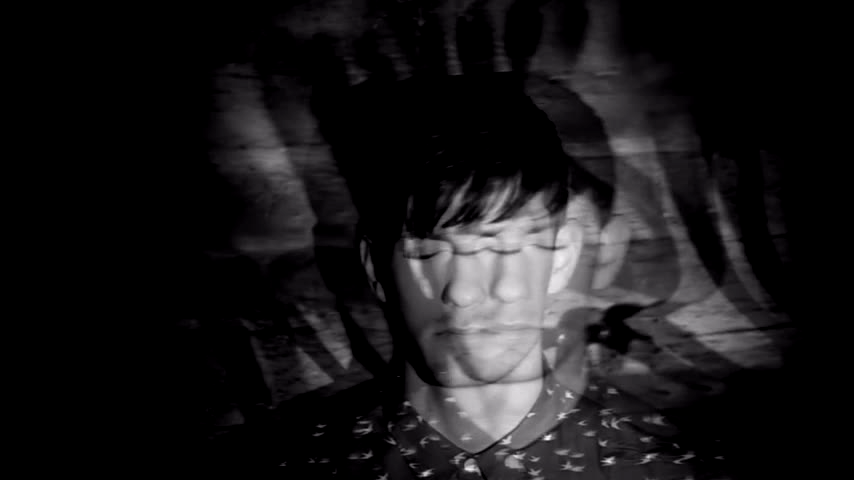
\includegraphics[width=\textwidth]{imagenes/whipLineal.png}
    \caption{Interpolador Lineal}
  \end{minipage}
\end{figure}

\newpage

\begin{figure}[h]
\centering
  \begin{minipage}[b]{.9\textwidth}
    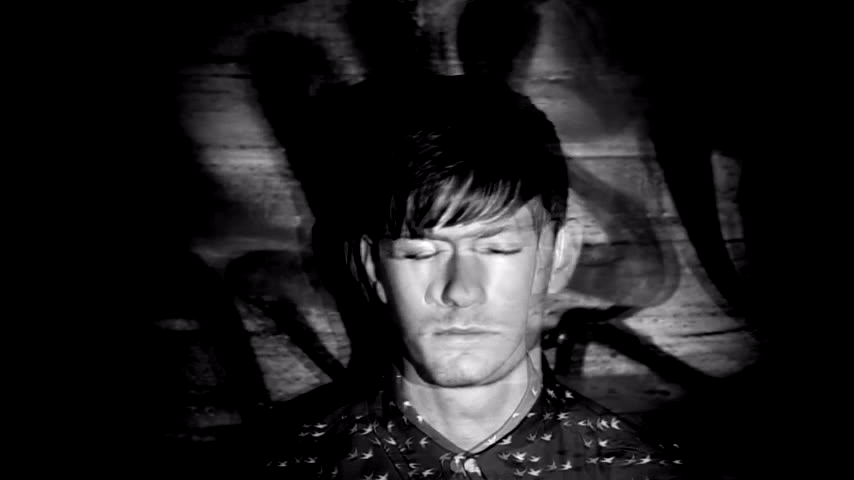
\includegraphics[width=\textwidth]{imagenes/whipSplines.png}
    \caption{Splines}
  \end{minipage}
\end{figure}

Como podemos apreciar, en el cuadro intermedio tenemos una "`fusion"' de los cuadros que se desea interpolar, esto es esperable debido a la forma que operan los metodos interpoladores. Consideramos que la principal razon de esta anomalia, es que se asume que cada pixel evoluciona de una manera particular para los cuadros intermedios (de manera lineal o cubica segun el interpolador), esto puede no darse en un video. Podemos apreciar esto en \texttt{whip\_pan.mp4}, en donde tenemos un objeto estatico frente a un fondo negro y podemos ver cuando la camara se desplaza en una direccion, el fondo negro se desplaza en direccion contraria de manera brusca, aqui tenemos pixeles que pasan a tener un valor cercano al cero de muy rapidamente, generando ghosting en los cuadros intermedios.

Si bien casos de cambios bruscos y contrastes fuertes son comunes en videos, tambien tenemos casos donde los pixeles del video evolucionan de manera mas acorde a los que generan los interpoladores. Uno de los casos idoneos para analizar esto es el video \texttt{zoom\_w\_dolly.mp4}, en donde tenemos por un lado un objeto que se mantiene relativamente estatico frente a un fondo que cambia bruscamente. El resultado lo podemos apreciar aqui:

\begin{figure}[h]
\centering
  \begin{minipage}[b]{.9\textwidth}
    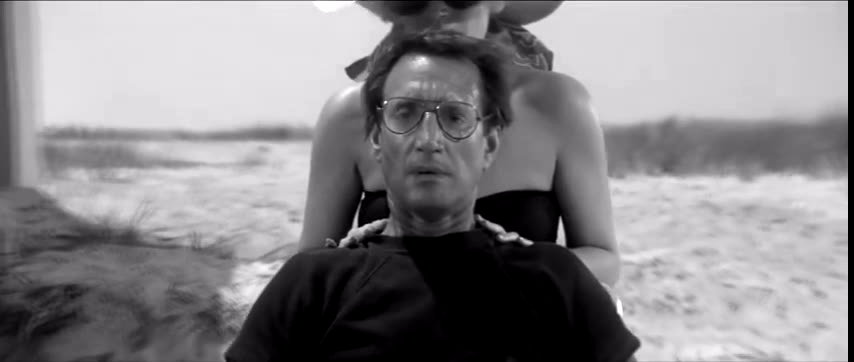
\includegraphics[width=\textwidth]{imagenes/zwdLineal.png}
    \caption{Interpolador Lineal}
  \end{minipage}
\end{figure}

\newpage

\begin{figure}[h]
\centering
  \begin{minipage}[b]{.9\textwidth}
    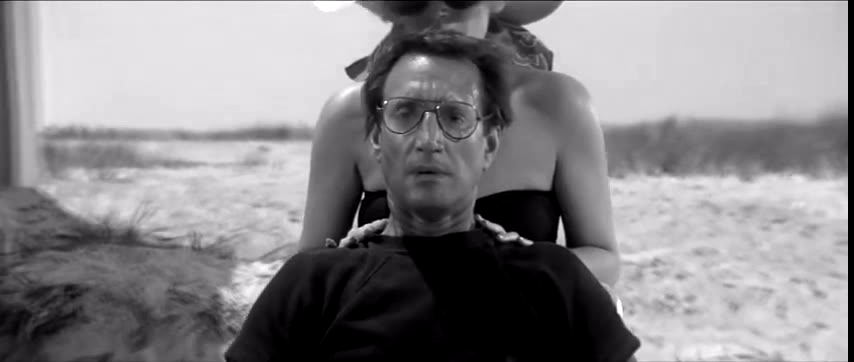
\includegraphics[width=\textwidth]{imagenes/zwdSplines.png}
    \caption{Splines}
  \end{minipage}
\end{figure}

En este caso se generaron dos cuadros intermedio, para mostrar la marcada diferencia entre el Interpolador Lineal y Splines. Como podemos apreciar, en el personaje estatico no se observan efectos de ghosting, sin embargo en el contorno del mismo y en el fondo (particularmente en las marcas de la arena) tenemos un efecto de ghosting, el cual es considerable en la interpolacion lineal, mientras que es ligero en la interpolacion con Splines cubicos. Es importante lo del contorno, ya que refuerza nuestra teoria de que los interpoladores no estan preparados para los cambios tan bruscos en los valores de un pixel en un intervalo de tiempo tan pequeño.

Por ultimo, vamos a anlizar lo ocurrido con las trancisiones bruscas, para ello utilizaremos el video \texttt{contrast\_cut.avi}. Aqui tenemos los resultados para el Interpolador Lineal y Splines:

\begin{figure}[h]
\centering
  \begin{minipage}[b]{.9\textwidth}
    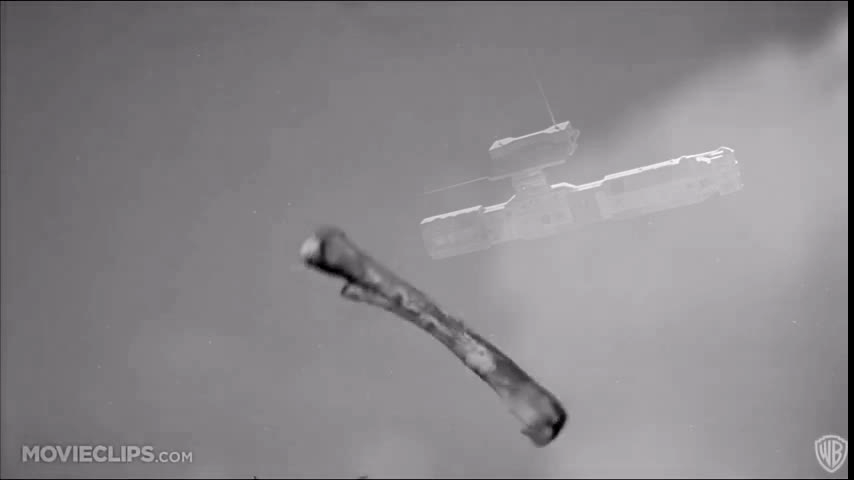
\includegraphics[width=\textwidth]{imagenes/ccutLineal.png}
    \caption{Interpolador Lineal}
  \end{minipage}
\end{figure}

\newpage

\begin{figure}[h]
\centering
  \begin{minipage}[b]{.9\textwidth}
    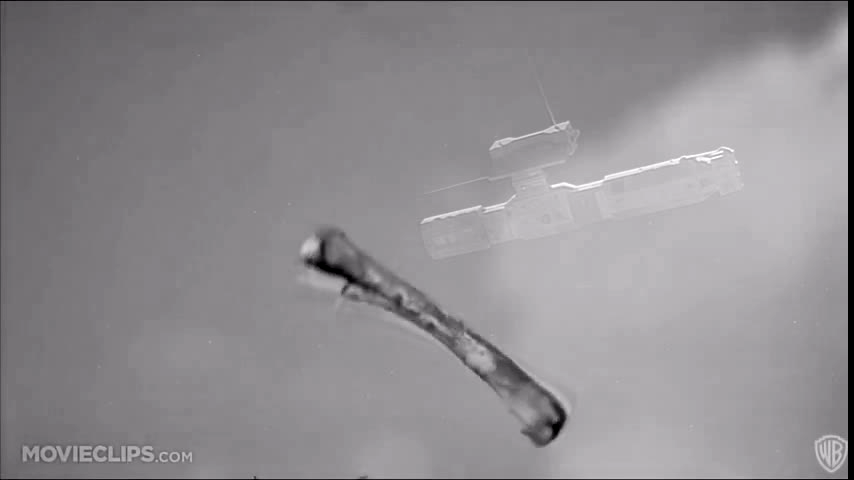
\includegraphics[width=\textwidth]{imagenes/ccutSplines.png}
    \caption{Splines}
  \end{minipage}
\end{figure}

Se puede ver que la imagen sufre un efecto de ghosting en ambos casos, para ambos metodos de interpolacion. Sin emabrgo, en este caso la fluidez de Splines le juega en contra respecto al metodo lineal, ya que este al tener anomalias visuales mucho mas presentes durante toda la duracion del video, el ghosting en la transicion no capta particularmente nuestra atencion. Splines, por otro lado, mantiene una suavidad mucho mas grande, con lo cual al encontrarnos con anomalias tan evidentes como en este caso, la reaccion que tenemos es mucho mas negativa.